% Episteme: a one-page scientific explainer.
% Build: cd docs && latexmk -pdf explainer.tex   (or: pdflatex explainer.tex)
\documentclass[10pt,twocolumn]{article}
\usepackage[a4paper,margin=13mm,columnsep=6.5mm]{geometry}
\usepackage[T1]{fontenc}
\usepackage{lmodern}
\usepackage{microtype}
\usepackage{amsmath}
\usepackage{xcolor}
\usepackage{tikz}
\usetikzlibrary{positioning,arrows.meta}
\usepackage{enumitem}
\usepackage{titlesec}
\usepackage{float}
\usepackage[hidelinks]{hyperref}

\definecolor{navy}{HTML}{0B1020}
\definecolor{blue}{HTML}{3D5AFE}
\definecolor{bluetint}{HTML}{E6EAFF}

\titleformat{\section}{\normalfont\bfseries\color{navy}}{\thesection}{0.6em}{}
\titlespacing*{\section}{0pt}{1.0ex plus .3ex}{0.4ex}
\setlist{nosep,leftmargin=1.1em}
\setlength{\parskip}{0.35ex}
\setlength{\parindent}{0pt}
\pagestyle{empty}
\raggedbottom


\begin{document}

\twocolumn[{%
  \begin{center}
    {\Large\bfseries\color{navy} Episteme: recording the reasons behind AI-assisted research}\\[0.6ex]
    {\small A provenance notebook for the AI4MetaScience hackathon (Task~2)}
  \end{center}
  \vspace{-0.6ex}
  \begin{quote}\small
    \textbf{Summary.} Research records keep results but lose the reasons that connect them. Episteme captures
    what a researcher and an AI agent do while the work happens, reduces that activity to a short diary of
    decisions, and labels each stated reason with who stated it. The design goal is a single test: when a study
    changes direction, a reviewer who was not present should be able to find out \emph{why} from the record
    alone, with every claim traceable to the evidence behind it.
  \end{quote}
  \vspace{0.4ex}
}]

\section{The problem}
A published study reports the path that worked. Failed expectations, abandoned runs and the moment someone
decided to try something else are rarely kept. Lab notebooks are usually written after the fact, from memory,
and seldom link a note to the exact code or output it describes. Reproducibility suffers: in a 2016 survey of 1{,}576 researchers, more than 70\% reported
having failed to reproduce another scientist's experiment (Baker, \emph{Nature} 533:452--454).

AI agents exacerbate the problem: an agent runs dozens of analyses in minutes, so the gap between what was done
and what was written down grows faster than anyone can close it by hand.

\section{Approach}
Episteme records while the work happens instead of reconstructing it later. Hooks in Claude Code and git send
every instruction, command, output and commit to a local, append-only \emph{raw log}. This log is complete but
too long to read, so it is segmented into \emph{episodes}: one instruction together with everything the agent
did in response. Simple rules turn each finished episode into a few \emph{diary entries}, and only the diary is
meant for people. Every entry keeps links to the raw events it came from.

\begin{center}
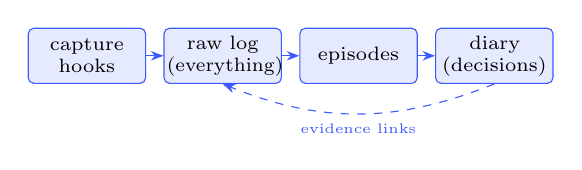
\begin{tikzpicture}[
  box/.style={draw=blue, fill=bluetint, rounded corners=2pt, align=center, font=\scriptsize,
              minimum height=7mm, inner sep=2pt, text width=13.5mm},
  arr/.style={-{Stealth[length=1.6mm]}, blue}, node distance=2.2mm]
  \node[box] (c) {capture\\ hooks};
  \node[box, right=of c] (r) {raw log\\ (everything)};
  \node[box, right=of r] (e) {episodes};
  \node[box, right=of e] (d) {diary\\ (decisions)};
  \draw[arr] (c) -- (r); \draw[arr] (r) -- (e); \draw[arr] (e) -- (d);
  \draw[arr, dashed] (d.south) to[bend left=22] node[below, font=\tiny] {evidence links} (r.south);
\end{tikzpicture}
\end{center}

\section{Five kinds of entry}
A researcher can add five kinds of entry by hand, and the capture rules produce the same kinds automatically.
\begin{description}[style=unboxed,leftmargin=0pt]
  \item[Thought.] A free-text note: a caveat, an idea, an observation. It needs no structure and costs one line.
  \item[Plan.] What will be tried next, optionally with a pre-stated expectation such as
        $\mathrm{AUROC}\ge 0.75$. Stating the expectation \emph{before} the run is what makes it testable.
  \item[Run.] An analysis that was carried out: the command, its result, its parameters, and whether it
        succeeded or failed. Scripts report results as plain \texttt{RESULT key=value} lines.
  \item[Surprise.] A result that contradicts what was expected. Surprises can be written by hand, but most are
        produced automatically (see below), so a broken expectation is never silently lost.
  \item[Artifact.] A durable output, typically a git commit, that fixes the state of the code at a point in
        the study.
\end{description}
A sixth kind, the \textbf{pivot}, is not entered directly. It marks a change of approach and is proposed by
Episteme when a new plan follows a surprise or a failed run.

\textbf{The expectation check.} Let a plan state an expectation $(m, \circ, v)$, a metric $m$, a comparison
$\circ \in \{\ge, \le, >, <\}$ and a threshold $v$. When the next run reports an observed value $x_m$, Episteme
evaluates $x_m \circ v$. If it is false, a surprise entry linking the plan and the run is recorded, without anyone
writing it down (steps 1--3 in Table~\ref{tab:demo}).

\section{Who stated the reason}
A record of reasons is only useful if it does not invent them. Every entry therefore carries an attribution:
stated by the \emph{researcher}, stated by the \emph{agent}, or \emph{inferred} by Episteme. When a language model
helps classify a possible pivot, a reason may be labelled as stated only if it appears as a verbatim quote in
the researcher's instruction or the agent's message; otherwise it is downgraded to inferred, and any model
paraphrase is stored separately and labelled as such. The researcher can confirm or correct a proposed reason
with one click. Without a model, everything except this classification still works.

\section{Answering the reviewer's question}
Table~\ref{tab:demo} shows the hospital-readmission demo, a simulated study predicting 30-day readmission from
clinical notes. At step~4 the study changes direction: it drops n-gram features for clinical embeddings. A
reader of the paper would see only the final model and ask \emph{why did they switch?} Because the pivot links
to the surprise that triggered it, and every entry links to its raw evidence, the answer is a lookup rather
than an act of memory. Episteme answers in plain language and cites entries: the plan expected $\mathrm{AUROC}\ge0.75$ but the run scored $0.54$
[E1--E3]; the researcher moved to clinical embeddings because n-grams ``lose the clinical semantics we need''
[E4]; the new approach reached $0.81$ [E5]. The diary also exports as a Markdown decision appendix for a paper,
or as W3C PROV-JSON for provenance tools.

\section{Scope and limits}
Episteme runs locally on the Python standard library and sends nothing off the machine unless a model is
connected. Capture covers Claude Code and git; other tools can post events over HTTP. Code and data versions are
not yet recorded per run, the rules that flag a pivot can miss subtle ones, and both demos are simulated.

\begin{table}[H]
\centering\scriptsize
\setlength{\tabcolsep}{3pt}
\begin{tabular}{@{}r l l l l@{}}
\hline
\# & id & kind & entry & who \\
\hline
1 & E1 & plan     & baseline, expects AUROC $\ge 0.75$ & researcher \\
2 & E2 & run      & \texttt{train\_tfidf.py}: AUROC $0.54$ & agent \\
3 & E3 & surprise & expected $\ge 0.75$, observed $0.54$ & inferred \\
4 & E7 & pivot    & n-grams $\to$ clinical embeddings & inferred$^\ast$ \\
5 & E4 & plan     & ``N-grams lose the clinical semantics\ldots'' & researcher \\
6 & E5 & run      & \texttt{embed\_pubmedbert.py}: AUROC $0.81$ & agent \\
7 & E6 & artifact & commit \texttt{a3f9c21} & agent \\
8 & E8 & thought  & caveat: one seed, one hospital & researcher \\
\hline
\end{tabular}
\caption{\small The first eight diary entries of the hospital-readmission demo. The pivot is E7 because it was
proposed after E4--E6 were written, then placed where the change happened. $^\ast$Awaiting the researcher's confirmation.}
\label{tab:demo}
\end{table}

\end{document}
